% use pdflatex -shell-escape slides.tex to compile
\documentclass[10pt]{beamer}
\usetheme[
%%% options passed to the outer theme
%    shownavsym          % show the navigation symbols
  ]{AAUsimple}
  
% If you want to change the colors of the various elements in the theme, edit and uncomment the following lines
% Change the bar and sidebar colors:
%\setbeamercolor{AAUsimple}{fg=red!20,bg=red}
%\setbeamercolor{sidebar}{bg=red!20}
% Change the color of the structural elements:
%\setbeamercolor{structure}{fg=red}
% Change the frame title text color:
%\setbeamercolor{frametitle}{fg=blue}
% Change the normal text color background:
%\setbeamercolor{normal text}{fg=black,bg=gray!10}
% ... and you can of course change a lot more - see the beamer user manual.
\usepackage{epstopdf}
\usepackage{movie15}
\usepackage[utf8]{inputenc}
\usepackage[english]{babel}
\usepackage[T1]{fontenc}
% Or whatever. Note that the encoding and the font should match. If T1
% does not look nice, try deleting the line with the fontenc.
\usepackage{helvet}
\usepackage[helvet]{sfmath}

% For math font script
\usepackage[mathscr]{euscript}

\usepackage{color, xcolor}
\usepackage{tikz}
% tikz setup for descendant robot motion figure 
\usetikzlibrary{positioning,chains,fit,shapes,calc}
\usetikzlibrary{arrows,shadows,trees}
\tikzset{
  basic/.style  = {draw, text width=2cm, drop shadow, font=\sffamily, rectangle},
  root/.style   = {basic, rounded corners=2pt, thin, align=center,
                   fill=red!30},
  level 2/.style = {basic, rounded corners=6pt, thin,align=center, fill=orange!30,
                   text width=8em},
  level 3/.style = {basic, thin, align=left, fill=pink!60, text width=8em}
}
% tikz setup for lattice graph
\usepackage{pgf}
\usetikzlibrary{automata}
\usepackage{hyperref}
\hypersetup{pdfpagemode=FullScreen}
\usepackage{ifthen}
\usepackage{animate}

% tikz animation
\usetikzlibrary{arrows,decorations.pathmorphing,through,backgrounds,positioning,fit,petri}
\usetikzlibrary{shapes.multipart}
\usetikzlibrary{decorations.pathreplacing}

\usepackage[tikz]{bclogo}

\newcommand{\id}{{\rm id}}
\newcommand{\edge}[3]{{#1}\overset{#2}{\longrightarrow}{#3}}

% colored hyperlinks
\newcommand{\chref}[2]{%
  \href{#1}{{\usebeamercolor[bg]{AAUsimple}#2}}%
}

\title{Distributed Formation of Arbitrary Lattice Pattern for
  Multi-robot Systems}

%\subtitle{v.\ 1.0.0}  % could also be a conference name
%\date{\today}
\author{
  Yang Song, Jason M. O'Kane\\
  \href{mailto:song24@email.sc.edu}{{\tt song24@email.sc.edu} \\
  \href{mailto:jokane@cse.sc.edu}{\tt jokane@cse.sc.edu}}
}

% - Give the names in the same order as they appear in the paper.
% - Use the \inst{?} command only if the authors have different
%   affiliation. See the beamer manual for an example

\institute[
%  {\includegraphics[scale=0.2]{aau_segl}}\\ %insert a company, department or university logo
  Dept.\ of Computer Science and Engineering\\
  University of South Carolina
] % optional - is placed in the bottom of the sidebar on every slide
{% is placed on the bottom of the title page
  Dept. of Computer Science and Engineering\\
  University of South Carolina
  
  %there must be an empty line above this line - otherwise some unwanted space is added between the university and the country (I do not know why;( )
}

% specify a logo on the titlepage (you can specify additional logos an include them in 
% institute command below
\pgfdeclareimage[height=1.5cm]{titlepagelogo}{sc_logo.pdf}%{aau_logo_new.pdf} % placed on the title page
%\pgfdeclareimage[height=1.5cm]{titlepagelogo2}{aau_logo_new.pdf} % placed on the title page
\titlegraphic{% is placed on the bottom of the title page
  \pgfuseimage{titlepagelogo}
%  \hspace{1cm}\pgfuseimage{titlepagelogo2}
}

\definecolor{scred}{RGB}{115,0,10}% dark red 
\definecolor{myblue}{RGB}{80,80,160}
\definecolor{mygreen}{RGB}{80,160,80}

\begin{document}
% the titlepage
\begin{frame}[plain] % the plain option removes the sidebar and header from the title page
  \titlepage
\end{frame}
%%%%%%%%%%%%%%%%
% TOC
% \begin{frame}{Agenda}{}
% \tableofcontents
% \end{frame}
%%%%%%%%%%%%%%%%

\section{Introduction}
\begin{frame}{Contribution}{}
\begin{block}{}
  \begin{columns}[T] % align columns
    \begin{column}{.48\textwidth}
      \begin{itemize}
      \item {\textcolor{scred}{\large WHAT DO WE HAVE:}}\\
        Given a set of autonomous robots, each robot knows its local information.
      \item {\textcolor{scred}{\large INPUT:}}\\
        Representations of various formation patterns.
      \item {\textcolor{scred}{\large OUTPUT:}}\\
        Robot motion control.
      \item {\textcolor{scred}{\large WHAT DO WE EXPECT:}}\\
        Various formation patterns.
      \end{itemize}
    \end{column}%
    \begin{column}{.48\textwidth}
      %% \begin{figure}
      \includemovie[poster,autoplay]{4cm}{4cm}{video.mp4}
      %% \end{figure}
      %\movie[externalviewer]{\beamergotobutton{Start movie}}{video.mp4}
    \end{column}%
  \end{columns}
  
\end{block}
\end{frame}
% motivation 

% \begin{frame}{Related Work}{}
%   \begin{block}{}
%     \begin{columns}[T] % align columns
%       \begin{column}{.48\textwidth}
%         \color{red}\rule{\linewidth}{4pt}
%         Left Part
%       \end{column}%
%       \hfill%
%       \begin{column}{.48\textwidth}
%         \color{blue}\rule{\linewidth}{4pt}
%         Right Part
%       \end{column}%
%     \end{columns}
% \end{block}
% \end{frame}

%%%%%%%%%%%%%%%%
\begin{frame}{Robot Specifications}{}
\begin{block}{}
  \begin{columns}[T] % align columns
      \begin{column}{.55\textwidth}
        \begin{itemize}
        \item Holonomic or Differential Drive robots.
        \item Each robot has an unique \textbf{ID}.
        \item Each robot has three states, use a vector $p = [x, y,
          \theta]^T$ to represent its \textbf{pose}.
        \item Each robot has a \textbf{range} within which it can
          sense and communicate with other robots.
        \item Each robot gets \textbf{observation} of its neighbors'
          IDs and relative poses in its body frame.
        \end{itemize}
      \end{column}%
      % right column
      \begin{column}{.45\textwidth}
        \begin{figure}
          \centering
          \begin{tikzpicture}[scale=0.55]
            \draw[violet, fill=violet!10] (3, 3) circle (3.2);
            \draw[fill=red] (3,3) -- (2.75,3) -- (3.25,3.25) -- (3,2.75)   	-- cycle;
            \node[color=red] at (3, 2.5) {$r_i$};
            
            \draw[color=red, dashed, ->] (1.5,1.5) -- (4.5,4.5) node[right] {$X^{(i)}$};
            \draw[color=red, dashed, ->] (4.5,1.5) -- (1.5,4.5) node[above] {$Y^{(i)}$};
            
            \draw[fill=blue!50] (0.5,4.5) -- (0.33,4) -- (0.5,4.125) -- (0.67,4) 	-- cycle;
            \node[color=blue] at (0.5,3.75) {$r_c$};
            \draw[fill=blue!50] (4,5) -- (3.75,5.5) -- (3.75,5.25) -- (3.5,5.25)   	-- cycle;
            \node[color=blue] at (3.5,5.7) {$r_f$};
            \draw[fill=blue!50] (1,2.5) -- (1.25,2) -- (1.25,2.25) -- (1.5,2.25)   	-- cycle;
            \node[color=blue] at (1.2,1.7) {$r_e$};
            \draw[fill=blue!50] (5,2.92) -- (4.5,2.75) -- (5,2.58) -- (4.875,2.75)  -- cycle;
            \node[color=blue] at (5.4,2.75) {$r_d$};
            % \draw[fill=blue!50] (-0.5,2.5) -- (-0.5,2.75) -- (-0.75,2.25) -- (-0.25,2.5)  -- cycle;
            % \node[color=blue] at (-0.75,3) {$r_b$};
          \end{tikzpicture}
          \caption{Robot $r_i$ and its neighbors $r_c, r_d, r_e,
            r_f$ in its local $X^{(i)}$-$Y^{(i)}$ coordinates. The
            disk describes $r_i$'s range.}
          \label{fig:robotmodel}
        \end{figure}
      \end{column}%
    \end{columns}
\end{block}
\end{frame}
%%%%%%%%%%%%%%%%

\section{Lattice Graph}
% definition of lattice graph
\begin{frame}{Lattice Graph}
    \begin{bclogo}[couleur=orange!10, arrondi=0.2, ombre=true]{Definition}
      A \textbf{lattice graph} is a strongly connected directed
      multigraph in which each edge $e$ is labeled with a rigid body
      transformation $T(e)$ and each $\edge{v}{T(e)}{w}$ has an
      inverse edge $\edge{w}{T(e)^{-1}}{v}$.  
    \end{bclogo}
    \begin{block}{}
%    \begin{bclogo}[couleur=orange!10, arrondi=0.2, ombre=true]{} 
      Given a lattice graph $G=(V, E)$ and a set of robots $R = \{
      r_1, \ldots, r_n \}$, we say that $R$ \textbf{satisfies} $G$ if
      there exists a role function $f: R \rightarrow V$ that preserves
      the neighborhood structure of $G$.
      % 
      Specifically, for any $i$ and $j$, if $r_i$ and $r_j$ are neighbors, 
      there must exist an edge
      $e_{ij}: \edge{f(r_i)}{}{f(r_j)}$ in $E$, such that
      $$ T(r_j) = T(r_i) T(e_{ij})$$
 %   \end{bclogo}
  \end{block}
\end{frame}

\begin{frame}{Lattice Graph}
    \begin{columns}[T] % align columns
      \begin{column}{.6\textwidth}
        \begin{block}{Example: lattice graph for repeated square patterns}
        \begin{itemize}
          \item  There is one node with four outgoing edges connecting to itself. 
          \item Each edge is associated with a translation $Tr(x, y)$
            of position $(x, y)$ relative to the current node.
          \item The edge length is $40$. 
          \item For a robot playing the role of this node, its
            neighbors should be in locations $(40, 0), (0, -40), (-40,
            0)$ and $(0, 40)$.
          \end{itemize}
        \end{block}
      \end{column}%
      \begin{column}{.4\textwidth}
        \begin{figure}
          \centering
          % \includegraphics[scale=0.45]{figs/sq}
          \begin{tikzpicture}[->,>=stealth',shorten >=5pt,auto,node distance=1cm,semithick]
            \tikzstyle{every state}=[fill=scred,draw=none, text=white]
            \node[state, scale=0.6] (A)         {$0$};
            \path (A) edge [loop above] node {Tr(0, 40)} (A)
                      edge [loop left]  node {Tr(-40,0)} (A)
                      edge [loop below] node {Tr(0, -40)} (A)
                      edge [loop right] node {Tr(40, 0)} (A);
          \end{tikzpicture}
        \end{figure}
        \begin{figure}
          \centering
          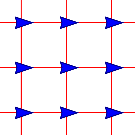
\includegraphics[scale=1]{figs/squarelattice}
        \end{figure}
      \end{column}%
    \end{columns}
\end{frame}

\subsection{Robot Authority}
\begin{frame}{Authority}
  \begin{block}{}
    \begin{bclogo}[couleur=orange!10, arrondi=0.2, ombre=true]{Definition} 
      An \textbf{authority} is an ordered list of robot IDs
      $$ \langle \id_1, \ldots, \id_k \rangle $$
      The first ID in the list, $\id_1$ is called the \textbf{root} ID.
      Likewise, the final ID in the list, $\id_k$ is called the
      \textbf{sender} ID.  The number $k$ of IDs in the list is called
      its \textbf{length}.
    \end{bclogo}
  \end{block}
  \begin{block}{Each robot broadcasts messages to its neighbors.}
    A message contains:\\
  \begin{itemize}
    \item The robot's authority.
    \item The robot's matching.
  \end{itemize}
  \end{block}
\end{frame}
%%%%%%%%%%%%%%%%

\subsection{Algorithm}
\begin{frame}{Algorithm}
  \begin{block}{General Algorithm Description}
    \begin{enumerate}
    \item<1-> Each robot decides whether to be a \textcolor{red}{root}
      robot or a \textcolor{blue}{descendant} robot based on ``authority''.
      
    \item<2-> Each robot chooses a \textcolor{purple}{role}. 
      \begin{itemize}
      \item \textcolor{red}{Root} robots always select the
        first lattice vertex as their role.  
      \item \textcolor{blue}{Descendant} robots accept
        their roles as from their parents.
      \end{itemize}    
      
    \item<3-> Each robot computes a local task assignment for
      its neighbors and broadcasts this assignment to its neighbors.
      
    \item<4-> Each \textcolor{blue}{descendant} robot moves toward to
      position assigned by its parent.
    \end{enumerate}
  \end{block}
\end{frame}
%%%%%%%%%%%%%%%%

% help me iron out the bugs or give me some comment and suggestions
\begin{frame}{Construct Authority Tree}{1. Decide to be root or descendant}
  \begin{block}{The key idea to make our local strategy reach a global static
    state is the authority carried by each robot}
    \begin{columns}[T] % align columns
      \begin{column}{.65\textwidth}
        \begin{itemize}
        \item Each robot chooses one of its neighbors to be its
          parent.
        \item Robots that choose not to select a parent are
          called \textbf{root} robot.
        \item Robots that select a parent are called
          \textbf{descendants} of that parent. 
        \end{itemize} 
        \hrule
        \begin{bclogo}[noborder=true, logo=\bccrayon]{} 
          Robot $4$ is the \textcolor{red}{Root} robot\\
          Robot $1$ is a descendant of Robot $4$\\
          Robot $2$ is a descendant of Robot $1$
        \end{bclogo}
        \hrule
      \end{column}%
      \begin{column}{.35\textwidth}
        \begin{figure}[center]
          \centering
          \begin{tikzpicture}[->,>=stealth',shorten >=1pt,auto,node distance=2cm,
            thick,main node/.style={circle,fill=red!20,draw,font=\sffamily}]

            \node[main node] (1) {1}; 
            \node[main node] (2) [below left of=1]
            {2}; 
            \node[main node] (4) [above left of=1] {4}; 
            \tikzset{node distance=1cm} 
            \node (11) [below of=1] {$\{4,1\}$}; 
            \node (22) [below of=2] {$\{4,1,2\}$}; 
            \node (44) [right of=4] {$\{4\}$}; 
            \path[every node/.style={font=\sffamily\small}] 
            (1) edge node[left] {} (2)            
            (4) edge node[right] {} (1);
          \end{tikzpicture}
        \end{figure} 
      \end{column}%
    \end{columns}
   \end{block} 
\end{frame}

\begin{frame}{Construct Authority Tree}{1. Decide to be root or descendant}
  \begin{block}{The robots use these authorities to establish a
      collection of authority trees}
    \begin{enumerate}
    \item Discards any message in which the authority contains its
      own ID.
    \item Forms an authority containing only its own ID,
      compares it with the authorities of remaining messages and
      selects the highest authority.
    \end{enumerate} 
  \begin{columns}[T] % align columns
    \begin{column}{.55\textwidth}
      \begin{itemize}
      \item If its authority is the highest, then it is
        the \textcolor{red}{root};
      \item Otherwise, it selects the one who sends the highest
        authority as its parent. Append its own ID to the highest
        authority to create its own authority. 
      \end{itemize}     
    \end{column}%
    \begin{column}{.45\textwidth}
      \begin{animateinline}[
        begin={%
          \begin{tikzpicture}%
            [demand2/.style={circle, fill=red!20!white, font=\tiny,
              text centered},%
            demand4/.style={circle, fill=green!20!white, font=\tiny,
              text centered},
            demand3/.style={circle, fill=blue!20!white, font=\tiny, text centered},
            post/.style={->,>=stealth', thin, draw=black!50},
            node/.style={circle,fill=red!20,draw,font=\sffamily\small}]%
            \useasboundingbox (-0.5,-0.5) rectangle (3.5,3);
          },
          end={\end{tikzpicture}}
        ]{10}
        \draw[red] (3,0) circle (2);  % color for 2: red
        \draw[green] (1,0) circle (2);   % color for 4: green
        \draw[blue] (3,2) circle (2);    % color for 3: blue
        \node (b) at (1,0) [demand4]  {4}; 
        \node (d) at (3,0) [demand2]  {2};
        \node (c) at (3,2) [demand3]  {3};
        \node (4) [above of=b] {(4)};
        \node (2) [above left of=d] {(2)};
        \node (3) [left of=c] {(3)};
        \newframe*
        \multiframe{10}{rP = 0.1 + .1, r = 1 + 1}{ 
          \draw[red] (3,0) circle (2);
          \draw[green] (1,0) circle (2);
          \draw[blue] (3,2) circle (2);
          \node (b) at (1,0) [demand4]  {4}; 
          \node (d) at (3,0) [demand2]  {2};
          \node (c) at (3,2) [demand3]  {3};
          % \path (b.east) -- (d.west) node[pos=\rP] (q){};
          % \draw[post] (b.east) -- (q.west);
          \node (4) [above of=b] {(4)};
          \node (2) [above left of=d] {(4,2)};
          \node (3) [left of=c] {(3)};
          % \path (d.north) -- (c.south) node[pos=\rP] (p){};
          % \draw[post] (d.north) -- (p.south);
        }
        \newframe*
        \multiframe{10}{rP = 0.1 + .1, r = 1 + 1}{ 
          \draw[red] (3,0) circle (2);
          \draw[green] (1,0) circle (2);
          \draw[blue] (3,2) circle (2);
          \node (b) at (1,0) [demand4]  {4}; 
          \node (d) at (3,0) [demand2]  {2};
          \node (c) at (3,2) [demand3]  {3};
          % \path (b.east) -- (d.west) node[pos=\rP] (q){};
          % \draw[post] (b.east) -- (q.west);
          \node (4) [above of=b] {(4)};
          \node (2) [above left of=d] {(4,2)};
          \node (3) [left of=c] {(4,2,3)};
          % \path (d.north) -- (c.south) node[pos=\rP] (p){};
          % \draw[post] (d.north) -- (p.south);
        }
        \newframe*
        \multiframe{10}{rP = 0.1 + .1, r = 1 + 1}{ %-->(PSD)
          \draw[red] (3,0) circle (2);
          \draw[green] (1,0) circle (2);
          \draw[blue] (3,2) circle (2);
          \node (b) at (1,0) [demand4]  {4}; 
          \node (d) at (3,0) [demand2]  {2};
          \node (c) at (3,2) [demand3]  {3};
          \path (b.east) -- (d.west) node[pos=\rP] (q){};
          \draw[post] (b.east) -- (q.west);
          %\path (b.east) edge (d.west);%%% edge without arrow
          \path (d.north) -- (c.south) node[pos=\rP] (p){};
          \draw[post] (d.north) -- (p.south);
          \node (4) [above of=b] {(4)};
          \node (2) [above left of=d] {(4,2)};
          \node (3) [left of=c] {(4,2,3)};
        }
      \end{animateinline}
    \end{column}
  \end{columns}
\end{block}
\end{frame}
%%%%%%%%%%%%%%%%

\begin{frame}{Construct Matching}{2. Role selection}
 \begin{block}{}
  Given a robot $r_i$ and a role vertex $v_i$ for that
  robot, let the lattice graph edge set $L=\{\emptyset,e_{ij}, e_{ik},
  \ldots\}$ be the set that contains a null value $\emptyset$ and all
  outgoing edges from vertex $v_i$. Let $Q=\{\id(r_a), \id(r_b),
  \ldots \}$ be the 
  \begin{columns}[T] % align columns
    \hspace{4mm}
    \begin{column}{.45\textwidth}
      set that contains the IDs of the neighbors of $r_i$.  
      \vspace{2mm}
      \hrule
      \hrule
     \begin{bclogo}[noborder=true, logo=\bccrayon]{} 
        A \textbf{matching} for a robot is a function $\eta : Q \rightarrow L$ that
        associates each neighbor ID with either a lattice graph edge
        from its role vertex or with the null value $\emptyset$.
      \end{bclogo}
      \hrule
      \hrule
    \end{column}%
    \begin{column}{.55\textwidth}
      \begin{figure}
        \centering
        \begin{tikzpicture}[
          fsnode/.style={},
          ssnode/.style={},
          every fit/.style={ellipse,draw,inner sep=0pt,text width=1cm},
          ->,shorten >= 2pt,shorten <= 2pt
          ]
          % the vertices of Q
          \begin{scope}[start chain=going below,node distance=1mm]
            \foreach \i/\xcoord in {1/\id(r_a),2/\id(r_b),3/\vdots, 4/\id(r_c)}
            \node[fsnode,on chain] (f\i) {$\xcoord$};
          \end{scope}
          % the vertices of L
          \begin{scope}[xshift=3cm,start chain=going below,node distance=1mm]
            \foreach \i/\xcoord in {5/e_{ij},6/e_{ik}, 7/\vdots, 8/\emptyset}
            \node[ssnode,on chain] (s\i) {$\xcoord$};
          \end{scope}         
          % the set U
          \node [myblue,fit=(f1) (f4),label=below:$Q$] {};
          % the set V
          \node [mygreen,fit=(s5) (s8),label=below:$L$] {};
          % the edges
          \draw (f1) -- (s6);
          \draw (f2) -- (s5);
          \draw (f4) -- (s8);
        \end{tikzpicture}
      \end{figure}
    \end{column}%
  \end{columns}
  \end{block}
\end{frame}
%%%%%%%%%%%%%%%%

% installation on Microsoft Windows Cont'd
\begin{frame}{Local Task Assignment}{3. Hungarain Algorithm}
  To compute an optimal matching of a robot with $N$ neighbors and $E$
  out-going edges of its role in the lattice graph, define a weight
  matrix of size $N \times \max(N, E)$ and apply
  \textcolor{scred}{Hungarian Algorithm}.
    \begin{columns}[T] % align columns
      \begin{column}{.5\textwidth}
        \begin{enumerate}
        \item Each row corresponds to a neighbor;
        \item Each column corresponds to an out-going edge of robot's
          role or a null value $\emptyset$.
        \item The entries of the matrix is the Euclidean distance
          between current position of each neighbor and the desired
          position if matched with a lattice graph edge.
        \end{enumerate}
      \end{column}%
      \begin{column}{.45\textwidth}
        \begin{figure}[center]
          \centering
          \begin{tikzpicture}[scale=0.6]
            \draw[fill=red] (3,3) -- (2.75,3) -- (3.25,3.25) -- (3,2.75)   	-- cycle;
            \node[color=red] at (3, 2.5) {$r_i$};
            \draw[color=red, dashed, ->] (1.5,1.5) -- (5,5) node[right] {$X^{(i)}$};
            \draw[color=red, dashed, ->] (4.5,1.5) -- (1,5) node[above] {$Y^{(i)}$};
            \draw[fill=blue!50] (0.5,4.5) -- (0.33,4) -- (0.5,4.125) -- (0.67,4) 	-- cycle;
            \node[color=blue] at (0.5,3.75) {$r_c$};
            \draw[fill=blue!50] (4,5) -- (3.75,5.5) -- (3.75,5.25) -- (3.5,5.25)   	-- cycle;
            \node[color=blue] at (3.5,5.7) {$r_f$};
            \draw[fill=blue!50] (1,2.5) -- (1.25,2) -- (1.25,2.25) -- (1.5,2.25)   	-- cycle;
            \node[color=blue] at (1.2,1.7) {$r_e$};
            \draw[fill=blue!50] (5,2.92) -- (4.5,2.75) -- (5,2.58) -- (4.875,2.75)  -- cycle;
            \node[color=blue] at (5.4,2.75) {$r_d$};
            \draw[fill=blue!50] (-0.5,2.5) -- (-0.5,2.75) -- (-0.75,2.25) -- (-0.25,2.5)  -- cycle;
            \node[color=blue] at (-0.75,3) {$r_b$};
            
            \draw[fill=red!40, dotted] (4,4) -- (3.75,4) -- (4.25,4.25) -- (4,3.75) -- cycle;
            \draw[fill=red!40, dotted] (2,2) -- (1.75,2) -- (2.25,2.25) -- (2,1.75) -- cycle;
            \draw[fill=red!40, dotted] (2,4) -- (1.75,4) -- (2.25,4.25) -- (2,3.75) -- cycle;
            \draw[fill=red!40, dotted] (4,2) -- (3.75,2) -- (4.25,2.25) -- (4,1.75) -- cycle;
            
            \draw[dashed](0.5, 4.25) -- (2,4);
            \draw[dashed](1.25,2.25) -- (2,2);
            \draw[dashed](3.75,5.25) -- (4,4);
            \draw[dashed](4.75,2.75) -- (4,2);
          \end{tikzpicture}
          \caption{Robot $r_i$ has its neighbors $r_c, r_d, r_e, r_f$
            match to one of its out-going edges, has $r_b$ match to $\emptyset$.}
        \end{figure}
      \end{column}%
    \end{columns}
\end{frame}
%%%%%%%%%%%%%%%%

\begin{frame}{Robot Motion Control}{4. Robot Movements}
  
  \textcolor{scred}{\large 1. Root Robot: Does Not Move}
  \begin{block}{2. Descendant Robot:}
    \begin{figure}
      \centering
      \begin{tikzpicture}[
        level 1/.style={sibling distance=40mm},
        edge from parent/.style={->,draw},
        >=latex]       
        % root of the the initial tree, level 1
        \node[root] {Descendant}
        % The first level, as children of the initial tree
        child {node[level 2] (c1) {Has matching with its parent}}
        child {node[level 2] (c3) {Has no matching with its parent}};
        % The second level, relatively positioned nodes
        \begin{scope}[every node/.style={level 3}]
          \node [below of = c1, xshift=10pt, yshift=-10pt] (c11) {Move
            towards its destination}; \node [below of = c11,
          yshift=-20pt] (c12) {Keep itself in the range of its
            parent}; \node [below of = c3, xshift=10pt, yshift=-10pt]
          (c31) {Move away from its parent}; \node [below of = c31,
          yshift=-20pt] (c32) { Discard any messages during
            movements};
        \end{scope}
        % lines from each level 1 node to every one of its "children"
        \foreach \value in {1,2}
        \draw[->] (c1.195) |- (c1\value.west);
        \foreach \value in {1,2}
        \draw[->] (c3.195) |- (c3\value.west);
      \end{tikzpicture}
    \end{figure}
  \end{block}
   
\end{frame}
%%%%%%%%%%%%%%%%
\begin{frame}{Robot Motion Control}{4. Constraints: Bounded Movement Model}
  \begin{block}{Bounded Movement Example}
    At time $t$, robot $r_i$ selects robot $r_p$ as its parent.
    \begin{columns}[T] % align columns
      \begin{column}{.5\textwidth}
      % Definition of circles
        \def\firstcircle{(0,0) circle (2cm)}
        \def\secondcircle{(2.3,1.8) circle (1.5cm)}
        \def\thirdcircle{(0,0) circle (1.5cm)}
        \colorlet{circle edge}{blue!50}
        \colorlet{circle area}{blue!20}
        \tikzset{filled/.style={fill=circle area, draw=circle edge, thick},
          outline/.style={draw=circle edge, thick}}
        \tikzstyle{important line}=[very thick]
        % Set A and B
        \begin{tikzpicture}[scale=0.65]
          \begin{scope}
            \clip \firstcircle;
            \fill[filled] \secondcircle;
          \end{scope}
          \draw[violet, fill=violet!10, dotted] (0, 0) circle (3.2cm);
          \draw[outline] \firstcircle node {$ $}; \draw[fill=circle
          area, red] (0,0) circle (0.1cm); \node at (-0.75,-0.3) {$p_p(t)$};
          \draw[style=important line, circle edge](90:1cm) --
          node[black]{$\phi- v\Delta{t}$}+(0,0); \draw[style=important
          line, circle edge](0,0) -- (135:2cm); \draw[outline]
          \secondcircle node {$ $};

          \draw[fill=circle area, blue] (2.3,1.8) circle (0.1cm); 
          \node at (3.2, 2) {$p_i^{(p)}(t)$};

          \draw[style=important line, circle edge](2.3, 1.8) -- (1.55,3.09);
          \node at (1.4, 2.2) {$v\Delta{t}$};

          \draw[fill=circle area, blue] (3, -0.7) circle (0.1cm); 
          \node at (3.8,-1) {$\bar{p}_i^{(p)}(t)$};
          \draw[dashed] \thirdcircle node{$ $};

          \draw[dashed](0, 0) -- (0,-1.5);
          \node at (0.5, -0.7) {$v\Delta{t}$};

          \draw[violet](0, 0) -- (-3.2, 0);
          \node at (-2.4, -0.5) {$\phi$};
          
          \draw[fill=circle area, blue] (1.96, 0.32) circle (0.1cm); \node
          at (3.5,0) {${p}_i^{(p)}(t+\Delta{t})$};
        \end{tikzpicture}
      \end{column}%
      \begin{column}{.45\textwidth}
        \begin{itemize}
        \item Shadowed region is the range of robot
          \textcolor{red}{$r_p$} at time $t$.
        \item The actual pose \textcolor{red}{$p_p(t+\Delta{t})$} of
          \textcolor{red}{$r_p$} could be anywhere in the dashed
          circle.
        \item The desired pose \textcolor{blue}{$\bar{p}_i^{(p)}(t)$}
          for robot \textcolor{blue}{$r_i$} is assigned by
          \textcolor{red}{$r_p$} at time $t$.
        \end{itemize}         
      \end{column}%
    \end{columns}
    On the boundary of the intersection of $P_p \cap P_i$,
    \textcolor{blue}{$r_i$} choose the nearest point to the desired
    ultimate destination position as its real destination position at
    time $t+\Delta{t}$
  \end{block}
\end{frame}
%%%%%%%%%%%%%%%%


\section{Results}
% \begin{frame}{Simulation and Experiments}{}
%   \begin{block}{}
%      \begin{columns}[T] % align columns
%       \begin{column}{.48\textwidth}
%         \color{red}\rule{\linewidth}{4pt}
%         Left Part
%       \end{column}
%       \begin{column}{.48\textwidth}
%         \begin{figure}
%           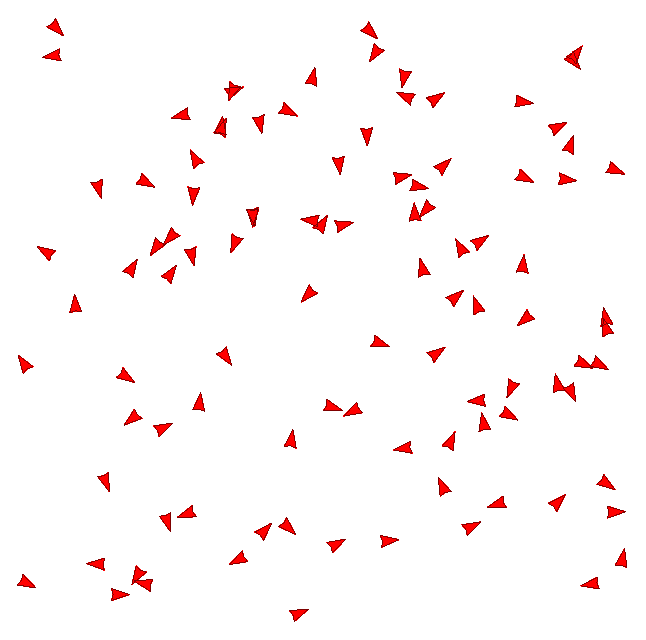
\includegraphics[scale=0.45]{figs/initial-formation}
%           \caption{Initial uniform distribution of $100$ robots's
%             poses.}
%         \end{figure}
%       \end{column}%
%     \end{columns}
%   \end{block}
% \end{frame}
%%%%%%%%%%%%%%%%
\begin{frame}{Simulation}{Octagon-square formation with 100 robots}
  \begin{block}{}
    \begin{columns}[T] % align columns
      \begin{column}{.5\textwidth}
         \begin{figure}
          \centering
           % 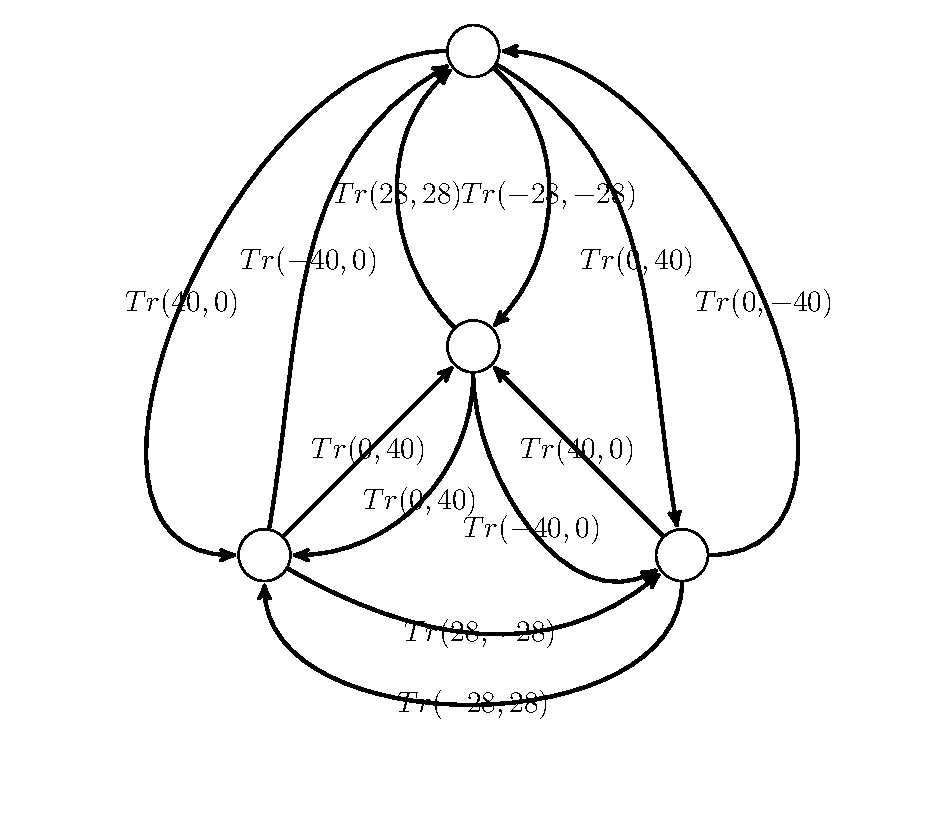
\includegraphics[width=.95\linewidth]{figs/octagonsquare}
            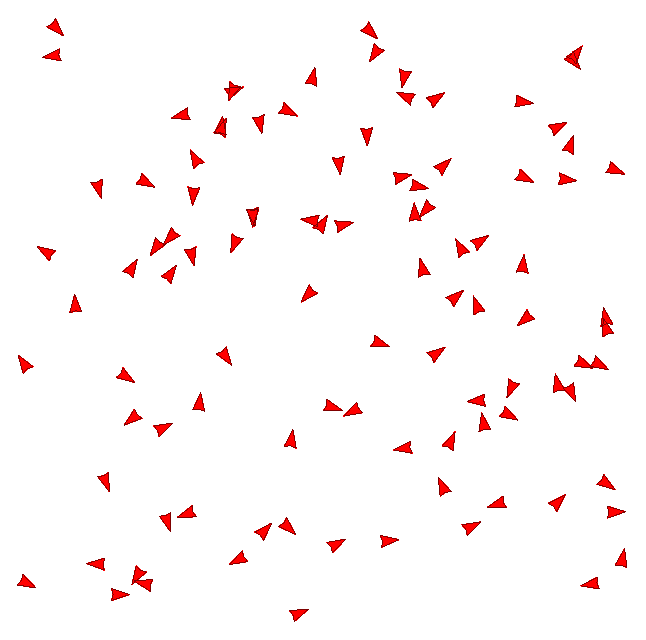
\includegraphics[scale=0.45]{figs/initial-formation}
            \caption{Initial uniform distribution of $100$ robots's
             poses.}
          \end{figure}
          \begin{center}
            %Lattice graph for repeated octagon-square pattern
          \end{center}
      \end{column}%
      \begin{column}{.5\textwidth}   
        \begin{figure}
          \centering
          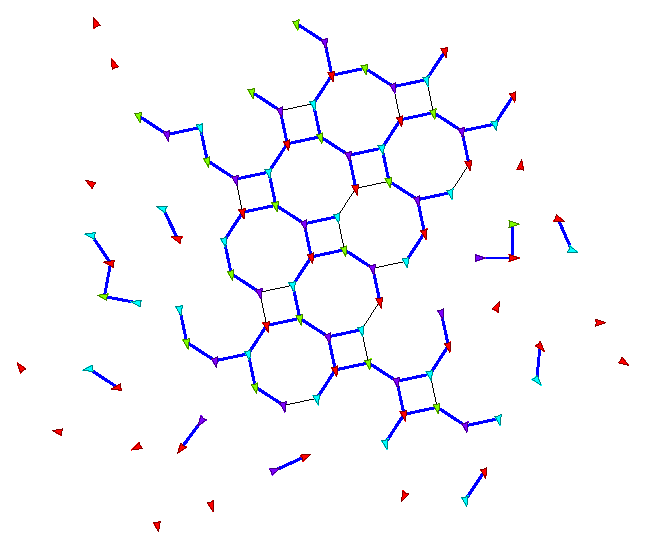
\includegraphics[width=\linewidth]{figs/final-formation}
          %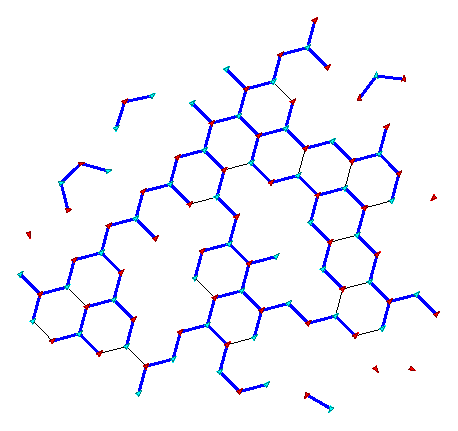
\includegraphics[width=.9\linewidth]{figs/formation-100}
          \caption{Final formation of repeated octagon-square pattern.}
        \end{figure}
        \begin{center}
%          Final formation.
        \end{center}
      \end{column}%
    \end{columns}
  \end{block}
\end{frame}
%%%%%%%%%%%%%%%%%%%%%%%%%%%%
\begin{frame}{Simulation}{Hexagon formation with 100 robots}
  \begin{block}{}
    \begin{columns}[T] % align columns
      \begin{column}{.5\textwidth}
        \begin{figure}
          \centering
          %
\includegraphics[scale=0.5]{figs/hex}
          %\caption{Lattice graph for repeated hexagon pattern}
          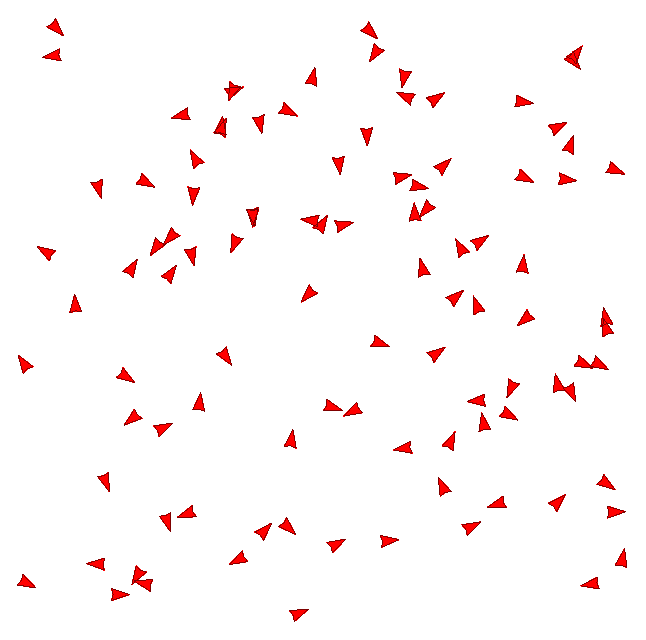
\includegraphics[scale=0.45]{figs/initial-formation}
          \caption{Initial uniform distribution of $100$ robots's
            poses.}
        \end{figure}
      \end{column}%
      \begin{column}{.5\textwidth}   
        \begin{figure}
            \centering
            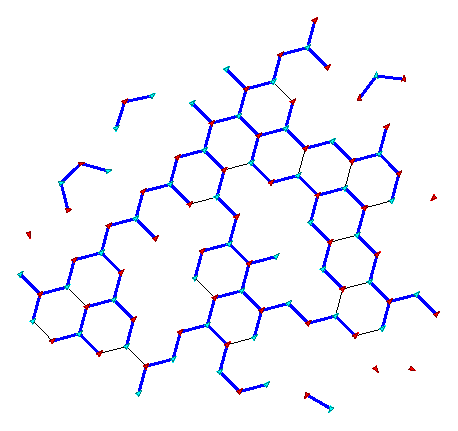
\includegraphics[width=0.85\linewidth]{figs/formation-100}
            \caption{Final formation of repeated hexagon pattern.}
        \end{figure}
      \end{column}%
    \end{columns}
  \end{block}
\end{frame}
%%%%%%%%%%%%%%%%

\begin{frame}{Experiments}{on three kinds of repeated
lattice patterns}
  \begin{block}{Experiments Setup}
    \begin{itemize}
    \item Keep a consistent velocity in all experiments
    \item Varied the number of robots $n=50, 100, 150, 200, 250$
    \item For each $n$, we repeated the experiment $50$ times
    \item Initially all robots are uniformly distributed with distinct
      random seeds each experiment
    \item For robustness test, randomly remove some robots from or add
      some robots to the system
    \end{itemize}
  \end{block}
  \begin{block}{Measurements}
    \begin{itemize}
    \item Average execution time
    \item Average non-fulfillment ratio: $\Gamma =
      \dfrac{1}{n}\sum\limits_{i=1}^n \frac{E_i - N_i}{E_i}$
    \end{itemize}
  \end{block}
\end{frame}

%%%%%%%%%%%%%%%%
% how to modify the theme
% {\setbeamercolor{AAUsimple}{fg=gray!50,bg=orange!50}
%  \setbeamercolor{structure}{fg=red}
%  \setbeamercolor{frametitle}{use=structure,fg=structure.fg}
%  \setbeamercolor{normal text}{bg=gray!20}
\begin{frame}{Results}{}
   \begin{columns}[T] % align columns
      \begin{column}{.48\textwidth}
        \begin{figure}
          \centering
          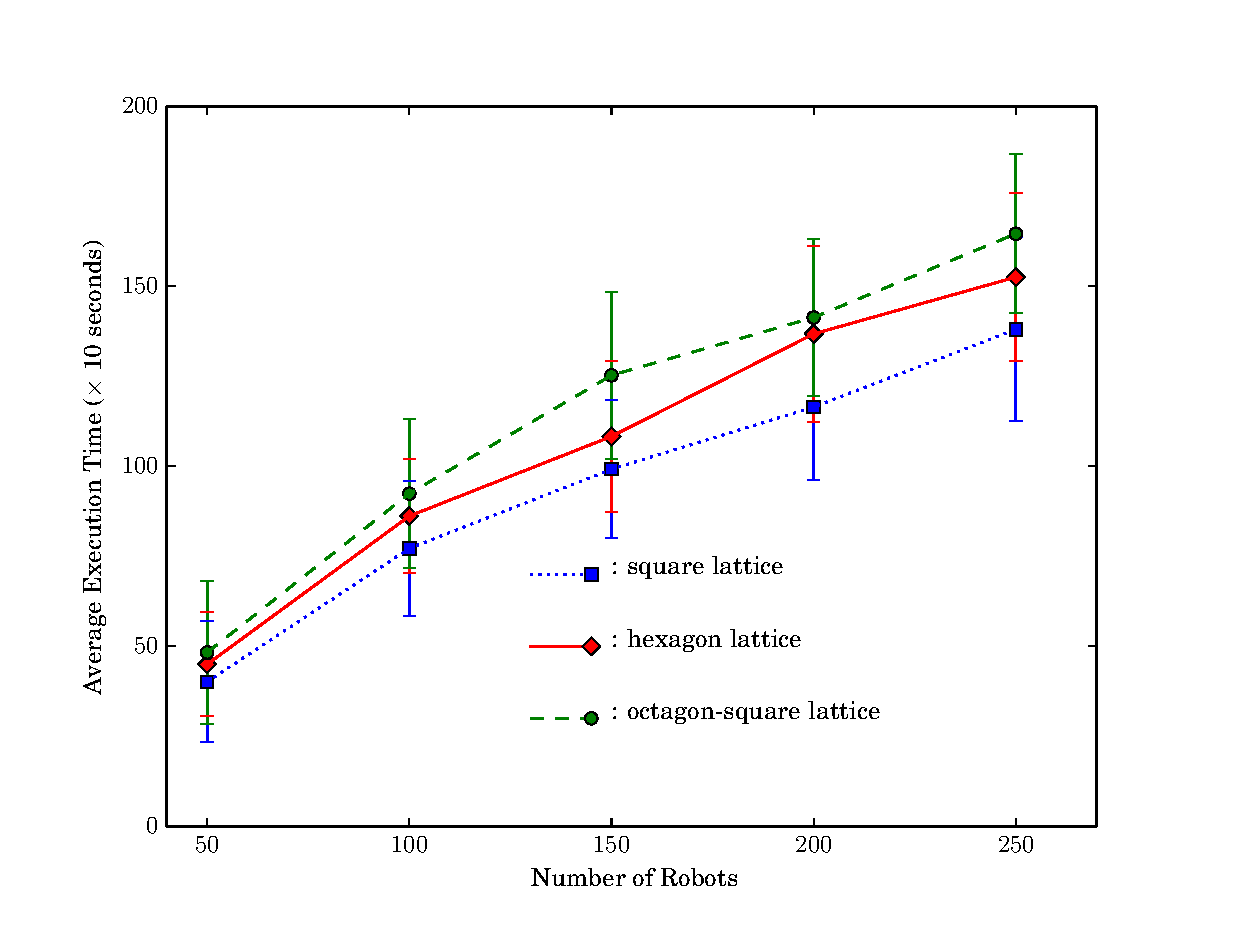
\includegraphics[width=\textwidth]{figs/exptime}
          \caption{Average execution time and its standard deviation
            of forming repeated lattice patterns of square, hexagon
            and octagon-square}
        \end{figure}
      \end{column}%
      \begin{column}{.48\textwidth}
        \begin{figure}
          \centering
          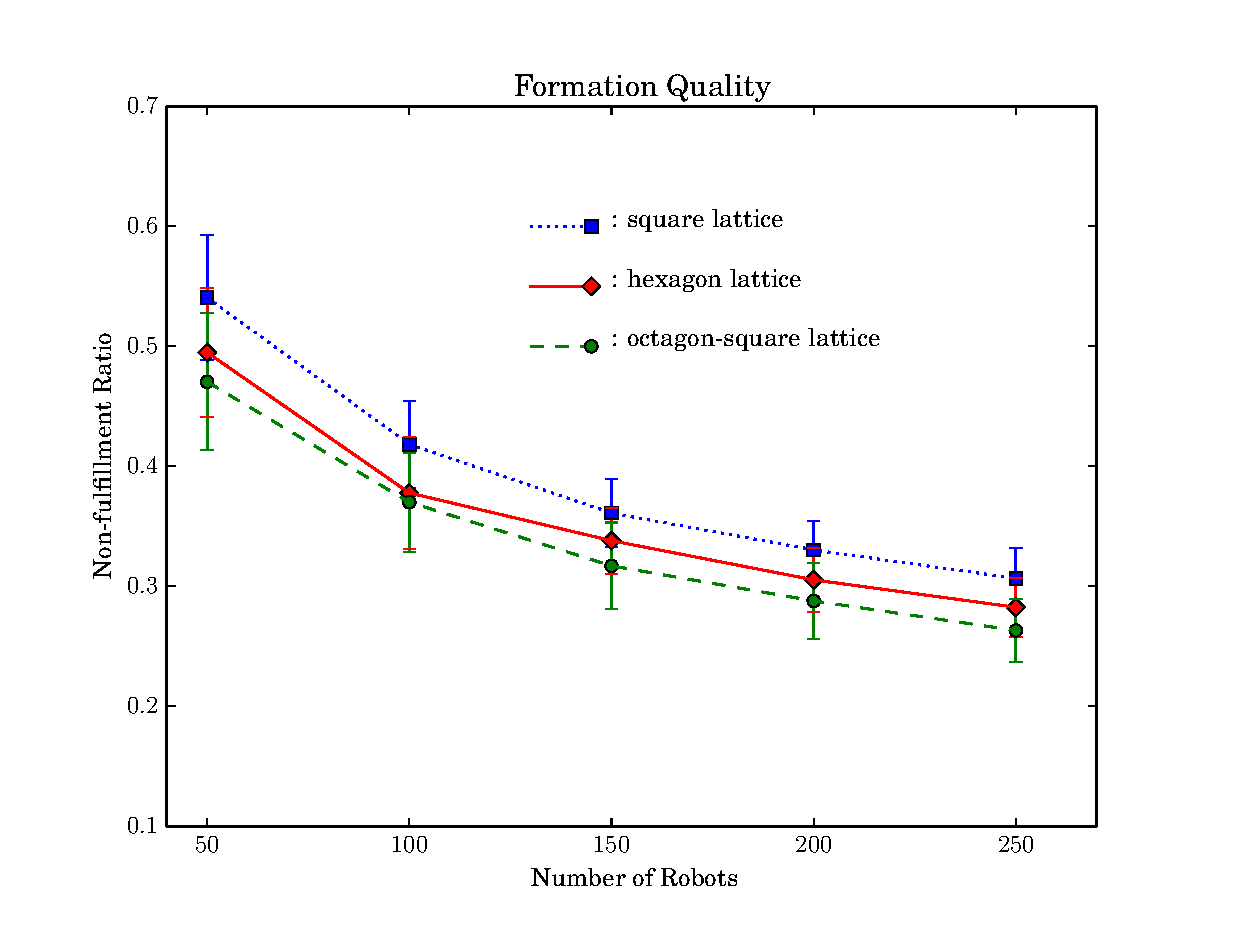
\includegraphics[width=\textwidth]{figs/expqual}
          \caption{Average non-fulfillment ratio and its standard
            deviation of forming lattice patterns of square, hexagon
            and octagon-square.}
        \end{figure}
      \end{column}%
    \end{columns}
\end{frame}
%%%%%%%%%%%%%%%%

\subsection{Conclusions}
% Widescreen Support
\begin{frame}{Conclusions}{}
\begin{block}{Pros of the Algorithm}
  \begin{itemize}
  \item robots can form different types of geometric formations,
including the repeated lattice patterns
  \item scales reasonably well with increasing numbers of robot
  \item robust to the situation when some robots are removed from or
with more robots added to the system
  \end{itemize}
\end{block}
\begin{block}{Cons of the Algorithm}
  \begin{itemize}
  \item no collision avoidance for motion strategy
  \item limited on the multi-robot systems subject to the nonholonomic
    constraints
  \end{itemize}
\end{block}
\end{frame}
%%%%%%%%%%%%%%%%


\subsection{Questions}
% contact information
\begin{frame}{Questions}{}
  \begin{center}
    \textcolor{scred}{\LARGE $\mathscr{THANK}$ $\mathscr{YOU}!$}
  \end{center}
\end{frame}
%%%%%%%%%%%%%%%%

\end{document}
